\chapter{Teknik Laboratorium III: Praktik Penelitian}\label{ch:b3:lab-techniques-3}

Sebotol larutan butillitium terbakar jika setetesnya bertemu dengan udara; sebuah
\omterm{def:b3:lab-techniques-3:schlenk}{kotak sarung tangan} menjaga oksigen dan air di bawah beberapa bagian per juta agar senyawa
semacam itu dapat ditimbang seperti garam dapur. Kimia penelitian sering dimulai dengan
menjauhkan atmosfer, dan berakhir dengan klaim yang harus dapat diperiksa orang lain:
sebuah senyawa baru, yang struktur dan kemurniannya dibuktikan dengan beberapa metode yang saling
bebas, dengan data yang dicatat dan diterbitkan agar pekerjaan itu dapat diulang. Bab
terakhir ini menghimpun praktik penelitian: menangani zat yang peka
udara, mengarakterisasi senyawa baru, menilai hasil secara statistik,
memelihara buku catatan dan membaca literatur, serta menilai risiko sebuah
prosedur yang belum pernah dijalankan siapa pun.

\begin{recall}
Jilid Tahun 1 membahas bahaya, risiko, piktogram, pernyataan H dan P, lembar data
keselamatan, dan ketidakpastian pengukuran beserta evaluasi tipe A dan tipe B-nya; Jilid
Tahun 2 membahas atmosfer inert, pengerjaan, zat pengering, kromatografi kilat,
spektrometri massa (HRMS, massa monoisotopik), NMR $^{13}$C, selang kepercayaan,
koefisien Student, kalibrasi, presisi, kebenaran, bias, keterulangan,
validasi metode, kenaikan suhu adiabatik, dan reaksi termal lepas kendali.
\Cref{ch:b3:advanced-nmr}, \cref{ch:b3:x-ray-diffraction}, dan
\cref{ch:b3:electrode-kinetics} menyediakan metode-metode struktur dan
elektrokimianya.
\end{recall}

\begin{omfigure}
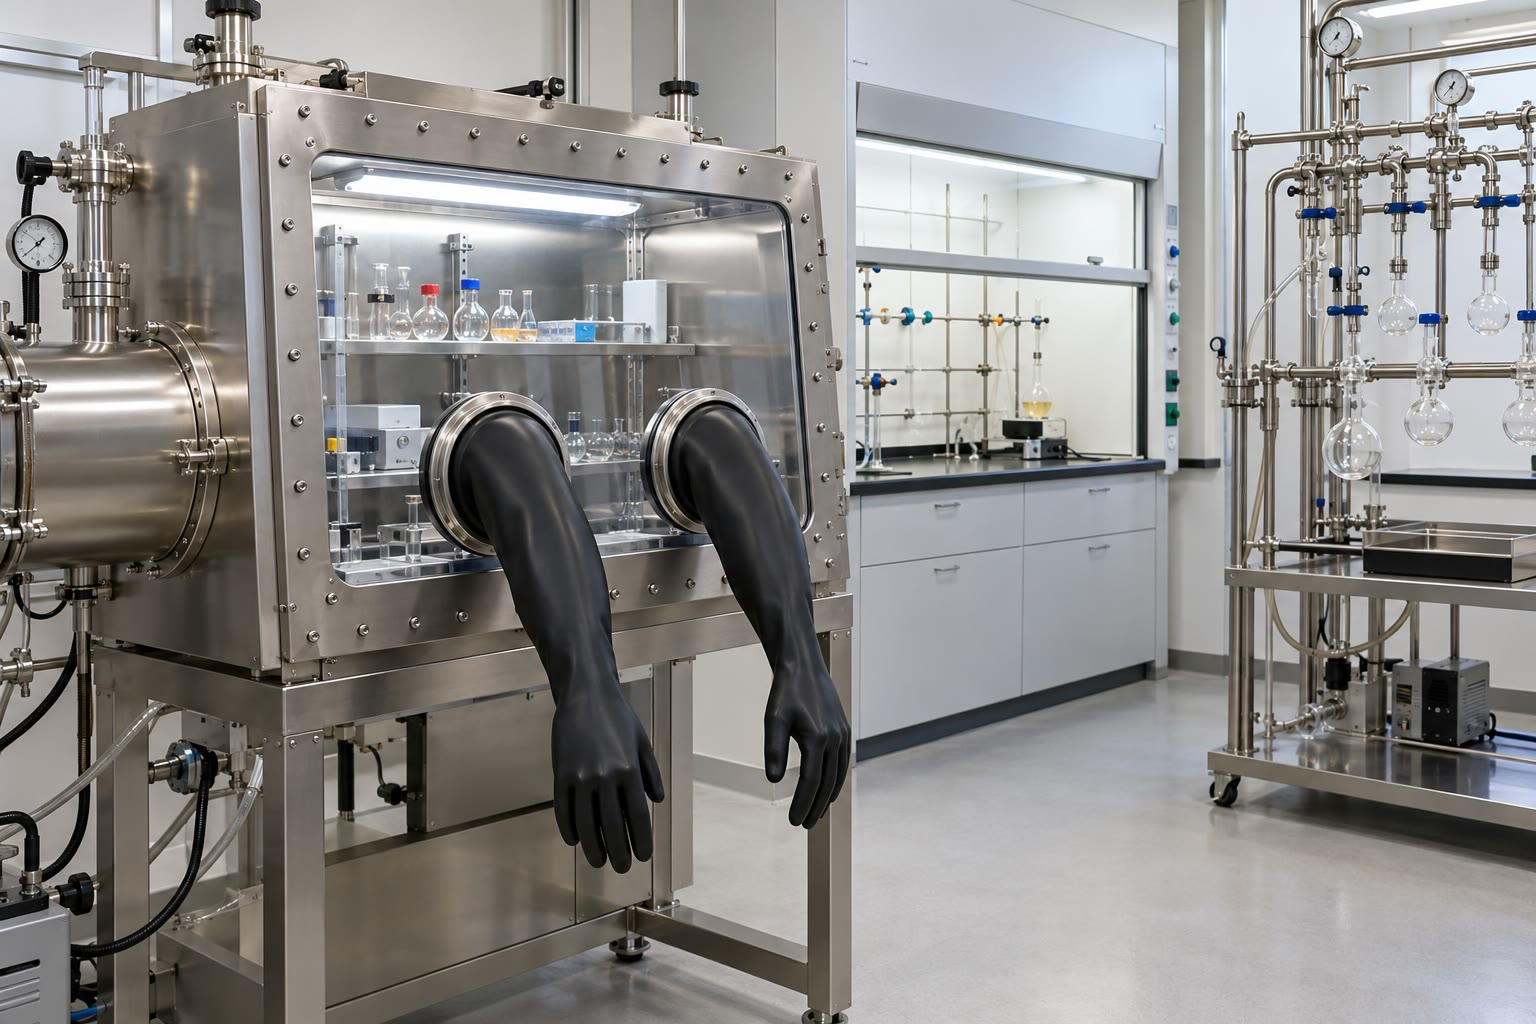
\includegraphics[width=0.58\linewidth]{images/book4/ai/b3-33-glovebox.jpg}

{\small Laboratorium penelitian dengan \omterm{def:b3:lab-techniques-3:schlenk}{kotak sarung tangan}: kotak baja tahan karat, yang diisi
nitrogen atau argon kering, dimasuki melalui sarung tangan; silinder di sebelah
kiri adalah ruang antara untuk memasukkan dan mengeluarkan barang.}
\end{omfigure}

\section{Bekerja tanpa udara}

\begin{definition}[Senyawa peka udara]\label{def:b3:lab-techniques-3:air-sensitive}
Yang disebut \emph{senyawa peka udara}\index{senyawa peka udara} adalah senyawa yang bereaksi dengan
dioksigen atau air di udara, sehingga terurai atau kehilangan aktivitasnya. Yang disebut
\emph{zat piroforik}\index{zat piroforik} adalah zat yang menyala dengan sendirinya di
udara.
\end{definition}

\begin{definition}[Jalur Schlenk dan kotak sarung tangan]\label{def:b3:lab-techniques-3:schlenk}
Yang disebut \emph{jalur Schlenk}\index{jalur Schlenk} adalah manifold kaca ganda, dengan satu tabung
yang terhubung ke pompa vakum melalui perangkap dingin, dan tabung lainnya ke pasokan gas inert kering
yang dibuang melalui gelembung minyak, dengan keran-keran yang menghubungkan setiap saluran ke
salah satunya. Yang disebut \emph{labu Schlenk}\index{labu Schlenk} adalah labu yang memiliki lengan samping berkeran
untuk dihubungkan ke jalur itu. Yang disebut \emph{kotak sarung tangan}\index{kotak sarung tangan} adalah kotak tertutup rapat
yang diisi gas inert, yang terus-menerus dimurnikan, tempat pekerjaan dilakukan melalui
sarung tangan.
\end{definition}

\begin{omfigure}
\begin{tikzpicture}[font=\scriptsize, >=Stealth]
  % manifold
  \draw[om glass, line width=1.1pt] (0,3.0) -- (8.0,3.0);
  \draw[om glass, line width=1.1pt] (0,2.5) -- (8.0,2.5);
  \node[anchor=east] at (-1.0,3.0) {gas inert};
  \node[anchor=east] at (0,2.5) {vakum};
  % keran
  \foreach \x in {2.0,4.0,6.0} {
    \draw[om glass] (\x,3.0) -- (\x,2.5);
    \draw[fill=white] (\x,2.75) circle (0.12);
    \draw (\x-0.1,2.75) -- (\x+0.1,2.75);
    \draw[om glass] (\x,2.5) -- (\x,2.0);
  }
  % labu pada keran tengah
  \draw[thick, black!60] (4.0,2.0) -- (4.0,1.6) -- (4.6,1.6);
  \pic[scale=0.5, transform shape] at (5.0,-0.2) {rbflask={0.3}{omDef!20}};
  \draw[om glass] (4.6,1.6) -- (4.9,1.25);
  \node[anchor=west] at (5.55,0.4) {labu Schlenk};
  % gelembung di ujung gas
  \pic[scale=0.55, transform shape] at (8.9,1.5) {bubbler};
  \draw[om glass] (8.0,3.0) -- (8.6,3.0) -- (8.6,2.9);
  \node[anchor=west] at (9.4,2.2) {gelembung minyak};
  % perangkap dan pompa di ujung vakum
  \draw[om glass] (0.4,2.5) -- (0.4,1.6);
  \draw[om glass, fill=omDef!8] (0.15,1.6) rectangle (0.65,0.4);
  \fill[omDef!25] (0.0,0.2) rectangle (0.8,1.2);
  \node[anchor=north] at (0.4,0.2) {perangkap dingin};
  \draw[om glass] (0.65,0.9) -- (1.6,0.9);
  \draw[fill=black!15] (1.6,0.6) rectangle (2.6,1.2);
  \node at (2.1,0.9) {pompa};
  \draw[->, thick] (-0.9,3.0) -- (0,3.0);
\end{tikzpicture}

{\small \omterm{def:b3:lab-techniques-3:schlenk}{Jalur Schlenk}, skematis: manifold gas dan manifold vakum yang dihubungkan oleh
keran-keran; setiap keran menghubungkan labunya ke vakum atau ke gas inert. Uap pelarut
yang tersedot mengembun di perangkap dingin sebelum mencapai pompa; gas keluar
melalui gelembung minyak, yang mencegah udara mengalir balik.}
\end{omfigure}

\begin{proposition}[Siklus pemvakuman--pengisian ulang]\label{prop:b3:lab-techniques-3:purge-cycles}
Jika sebuah labu berisi udara pada tekanan $p_0$ divakumkan sampai $p_{\min}$ lalu diisi kembali dengan
gas inert murni, sebanyak $n$ kali, fraksi udara awal yang tersisa adalah $(p_{\min}/p_0)^n$.
\end{proposition}

\begin{proof}
Pemvakuman sampai $p_{\min}$ menyisakan fraksi gas sebesar $p_{\min}/p_0$, dengan komposisi yang sama; pengisian
ulang dengan gas inert murni memulihkan $p_0$ tanpa menambahkan udara. Setiap siklus mengalikan
fraksi udara dengan $p_{\min}/p_0$; setelah $n$ siklus, $(p_{\min}/p_0)^n$.
\end{proof}

Tiga siklus sampai \qty{0.1}{mbar} di atas kertas menyisakan $10^{-12}$ udara; dalam praktik, kebocoran, gas
yang teradsorpsi pada kaca, serta pelepasan gas dari gemuk dan septum menentukan batasnya, dan itulah
sebabnya peralatan kaca dikeringkan dalam oven dan dirakit selagi panas.

\begin{definition}[Transfer kanula]\label{def:b3:lab-techniques-3:cannula}
Yang disebut \emph{transfer kanula}\index{transfer kanula} adalah pemindahan cairan yang peka udara
dari satu bejana tertutup ke bejana lain melalui jarum panjang berujung ganda, yang didorong
oleh tekanan lebih gas inert yang kecil di dalam bejana pertama.
\end{definition}

\begin{omfigure}
\begin{tikzpicture}[font=\scriptsize, >=Stealth]
  \pic at (0,0) {rbflask={0.35}{omThm!25}};
  \pic at (4.2,0) {rbflask={0.1}{omDef!15}};
  \pic at (0,3.0) {septum};
  \pic at (4.2,3.0) {septum};
  \draw[black!70, line width=0.9pt] (0.05,0.25) -- (0.05,3.5) to[out=90, in=90] (4.15,3.5) -- (4.15,1.6);
  \draw[->, thick, omThm] (1.3,3.95) -- (2.9,3.95) node[midway, above] {cairan};
  \draw[->, thick] (-1.3,3.4) -- (-0.15,3.2) node[pos=0, left] {gas inert masuk (tekanan sedikit lebih)};
  \draw[->, thick] (4.35,3.2) -- (5.4,3.6) node[right] {dibuang ke gelembung};
  \node[anchor=north] at (0,-0.1) {sumber};
  \node[anchor=north] at (4.2,-0.1) {penerima};
\end{tikzpicture}

{\small \omterm{def:b3:lab-techniques-3:cannula}{Transfer kanula}: ujung bawah kanula tercelup di dalam cairan labu
sumber; gas inert yang dimasukkan ke dalam sumber mendorong cairan melalui
kanula ke dalam labu penerima, yang dibuang melalui sebuah jarum ke gelembung.}
\end{omfigure}

\begin{method}[Sebuah transfer kanula]\label{met:b3:lab-techniques-3:cannula}
\begin{enumerate}
  \item Tempatkan kedua labu, yang ditutup septum, di bawah gas inert pada \omterm{def:b3:lab-techniques-3:schlenk}{jalur Schlenk}.
  \item Bilaslah kanula dengan gas: tusukkan satu ujungnya ke dalam sumber di atas cairan
        sampai gas mengalir keluar dari ujung yang lain, lalu tusukkan ujung itu ke dalam penerima.
  \item Buat saluran buang pada penerima dengan sebuah jarum; dorong ujung kanula di sisi sumber ke bawah
        permukaan cairan: tekanan lebih itu mendorong cairan menyeberang.
  \item Untuk menghentikan, angkat ujungnya ke atas cairan; cabut kanula dari penerima
        lebih dahulu, dan segera bilas kanula dengan pelarut kering, lalu dengan air, di dalam lemari asam.
\end{enumerate}
\end{method}

\begin{definition}[Penghilangan gas beku--pompa--cair]\label{def:b3:lab-techniques-3:degassing}
Yang disebut \emph{penghilangan gas beku--pompa--cair}\index{penghilangan gas beku--pompa--cair} adalah cara
menyingkirkan gas terlarut dari cairan dengan membekukannya dalam nitrogen cair, memvakumkan
ruang di atasnya, menutup keran, dan membiarkannya mencair, sehingga gas terlarut lepas
ke dalam vakum; siklus itu diulang tiga kali.
\end{definition}

Pelarut kering kini diperoleh dari kolom alumina teraktivasi di bawah gas inert
alih-alih dari alat distilasi di atas natrium. Larutan organolitium melemah seiring
waktu dan dititrasi sebelum dipakai, misalnya terhadap sejumlah asam
difenilasetat yang ditimbang dalam THF kering: ekuivalen pertama mendeprotonasi asam itu, dan
tetes kelebihan pertama memberikan dianion yang berwarna kuning.

\begin{proposition}[Titer organolitium]\label{prop:b3:lab-techniques-3:titre}
Jika massa $m$ asam difenilasetat (massa molar $M$) memerlukan volume $V$ larutan
organolitium untuk mencapai perubahan warna, konsentrasinya adalah $c = m/(MV)$.
\end{proposition}

\begin{proof}
Sampai titik akhir, setiap organolitium mengambil satu proton dari asam; warnanya
muncul ketika asamnya habis terpakai. Jumlah keduanya sama: $cV = m/M$.
\end{proof}

\begin{inthelab}[Ruang antara kotak sarung tangan]
Barang-barang masuk ke dalam \omterm{def:b3:lab-techniques-3:schlenk}{kotak sarung tangan} melalui ruang antaranya: barang itu ditempatkan di dalamnya,
pintu luar ditutup, dan ruang itu divakumkan lalu diisi kembali dengan gas kotak
tiga kali, dengan pemvakuman akhir yang lama untuk barang berpori, yang menahan udara;
baru kemudian pintu dalam dibuka dari dalam kotak dengan sarung tangan. Pelarut
dan wadah terbuka berisi cairan atsiri tidak pernah divakumkan di ruang antara, dan
tidak ada zat yang akan meracuni pemurni (tiol, pelarut terhalogenasi) yang dibuka
di dalam kotak tanpa izin.
\end{inthelab}

\begin{omfigure}
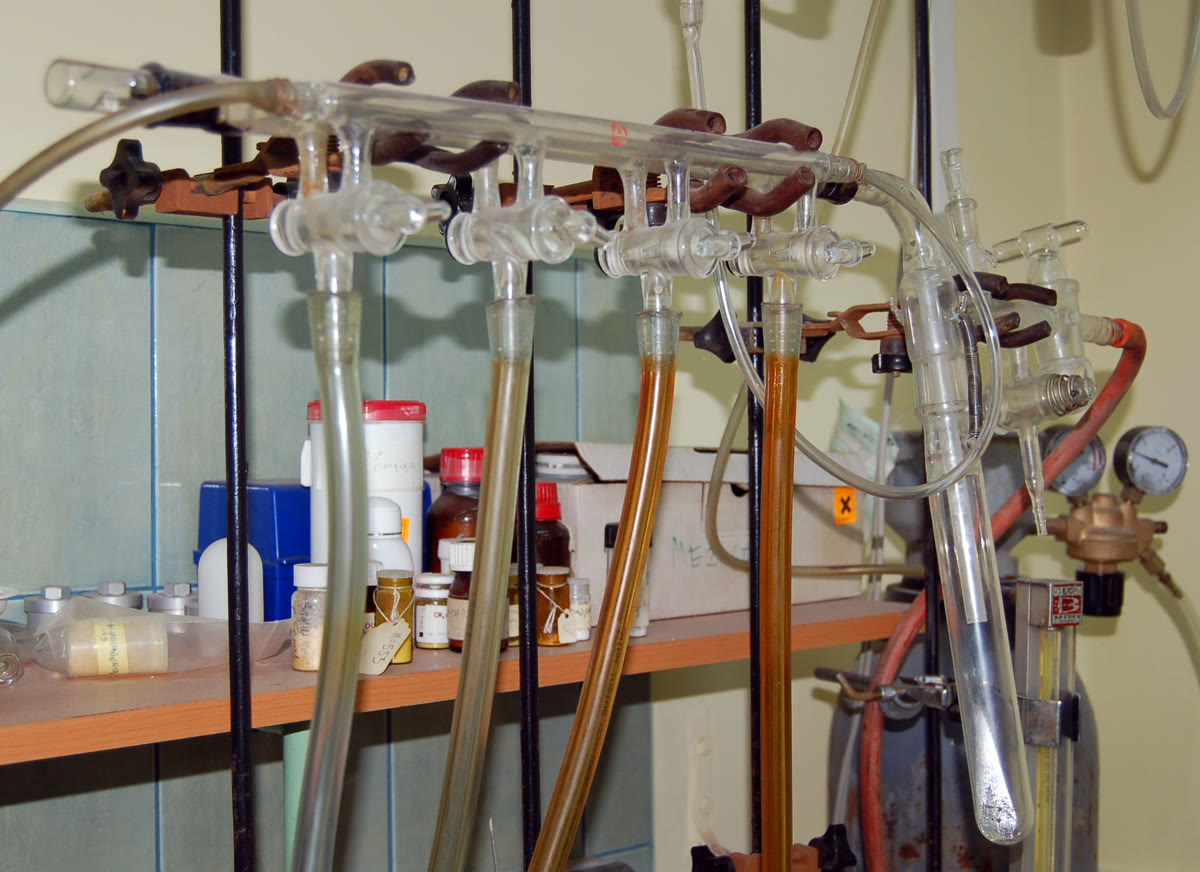
\includegraphics[width=0.46\linewidth]{images/book4/schlenk-line.jpg}

{\small \omterm{def:b3:lab-techniques-3:schlenk}{Jalur Schlenk} yang sedang dipakai: manifold kaca dengan keran-kerannya, selang ke
labu-labu, dan regulator gas. Foto: Polimerek, CC BY-SA 3.0.}
\end{omfigure}

\section{Mengarakterisasi senyawa baru}

\begin{method}[Mengarakterisasi senyawa baru]\label{met:b3:lab-techniques-3:characterise}
\begin{enumerate}
  \item Kemurnian: satu noda pada KLT dengan dua eluen, satu puncak pada HPLC atau GC, titik
        leleh yang tajam; \omterm{def:b3:lab-techniques-3:qnmr}{NMR kuantitatif} jika diperlukan kemurnian massa.
  \item Rumus: HRMS dalam batas beberapa ppm dari massa yang dihitung, beserta pola
        isotopnya; atau \omterm{def:b3:lab-techniques-3:elemental}{analisis unsur}.
  \item Struktur: NMR $^1$H dan $^{13}$C dengan percobaan 2D untuk hubungan-hubungannya
        (\cref{ch:b3:advanced-nmr}), IR untuk gugus-gugus fungsi; struktur sinar-X
        kristal tunggal jika kristal dapat tumbuh (\cref{ch:b3:x-ray-diffraction}).
  \item Stereokimia: NOE, tetapan kopling, rotasi optis, ee dengan kromatografi
        kiral.
  \item Laporkan setiap data beserta kondisinya, dan spektrum-spektrumnya dalam \omterm{def:b3:lab-techniques-3:literature}{informasi
        pendukung}.
\end{enumerate}
\end{method}

\begin{omfigure}
\begin{tikzpicture}[font=\scriptsize, >=Stealth,
  box/.style={draw, rounded corners, align=center, fill=omDef!8, inner sep=3pt, minimum height=8mm}]
  \node[box] (a) at (0,0) {senyawa baru\\ diisolasi};
  \node[box] (b) at (2.85,0) {murni?\\ KLT, HPLC, t.l.};
  \node[box] (c) at (5.85,0) {rumus\\ HRMS, CHN};
  \node[box] (d) at (8.75,0) {struktur\\ NMR (1D, 2D), IR};
  \node[box] (e) at (8.75,-1.6) {sinar-X jika\\ ada kristal,\\ stereokimia};
  \node[box, fill=omMeth!12] (f) at (5.85,-1.6) {konsisten?\\ laporkan dengan\\ data mentah};
  \node[box, fill=omThm!10] (g) at (2.85,-1.6) {murnikan lagi\\ (kromatografi,\\ kristalisasi)};
  \draw[->, thick] (a) -- (b); \draw[->, thick] (b) -- node[above, inner sep=1pt] {ya} (c);
  \draw[->, thick] (c) -- (d); \draw[->, thick] (d) -- (e); \draw[->, thick] (e) -- (f);
  \draw[->, thick] (b) -- node[left] {tidak} (g); \draw[->, thick] (g.north west) to[bend left=30] (a.south);
\end{tikzpicture}

{\small Alur kerja karakterisasi senyawa baru: kemurnian lebih dahulu, lalu
rumus, lalu struktur; setiap klaim bertumpu pada sedikitnya dua metode yang saling
bebas, dan \omterm{def:b3:lab-techniques-3:notebook}{data mentahnya} disertakan bersama laporan.}
\end{omfigure}

\begin{definition}[Analisis unsur]\label{def:b3:lab-techniques-3:elemental}
Yang disebut \emph{analisis unsur}\index{analisis unsur} (analisis pembakaran) adalah penentuan
persen massa karbon, hidrogen, nitrogen, dan belerang dalam sebuah
sampel dengan membakarnya dalam oksigen dan mengukur karbon dioksida, air,
dinitrogen, dan belerang dioksida yang terbentuk.
\end{definition}

\begin{proposition}[Persen massa dari rumus]\label{prop:b3:lab-techniques-3:mass-fractions}
Untuk rumus $\mathrm{C}_a\mathrm{H}_b\mathrm{N}_c\dots$ dengan massa molar $M$, persen massa karbon adalah $100\,aA_r(\mathrm C)/M$, dan demikian pula
untuk unsur-unsur lainnya.
\end{proposition}

\begin{proof}
Satu mol senyawa, dengan massa $M$, mengandung $a$ mol atom karbon, dengan massa $aA_r(\mathrm C)$;
rasionya, dikalikan 100, adalah persen massa.
\end{proof}

% ledger: ea:tolerance, hrms:tolerance
Sebagian besar jurnal kimia meminta nilai C, H, dan N yang ditemukan berada dalam batas 0.4 poin
persentase dari nilai yang dihitung, atau pengukuran HRMS dalam batas beberapa ppm (5 ppm
untuk sebagian jurnal), sebagai bukti komposisi. Sebuah studi antarlaboratorium yang besar mendapati bahwa
bahkan sampel murni cukup sering tidak memenuhi kriteria 0.4, sebuah pengingat bahwa sebuah
kriteria bukanlah hukum alam.

\begin{proposition}[Galat HRMS]\label{prop:b3:lab-techniques-3:ppm-error}
Galat massa terukur $m_{\mathrm{meas}}$ terhadap massa terhitung $m_{\mathrm{calc}}$ adalah
$10^6(m_{\mathrm{meas}} - m_{\mathrm{calc}})/m_{\mathrm{calc}}$ ppm; untuk sebuah ion, $m_{\mathrm{calc}}$ dihitung dari massa monoisotopik dikurangi (atau ditambah)
massa elektron yang dilepaskan (atau ditambahkan).
\end{proposition}

\begin{proof}[Menurut definisi]
Galat ppm adalah selisih relatif yang dinyatakan dalam bagian per juta; massa
ion berbeda dari massa rumus netralnya sebesar massa elektron, masing-masing \qty{5.486e-4}{u}, yaitu
beberapa ppm pada massa beberapa ratus.
\end{proof}

\begin{definition}[NMR kuantitatif]\label{def:b3:lab-techniques-3:qnmr}
Yang disebut \emph{NMR kuantitatif}\index{NMR kuantitatif} (qNMR) adalah penentuan jumlah atau
kemurnian dari integral sinyal, yang sebanding dengan jumlah inti
jika spektrumnya direkam dengan relaksasi penuh di antara pulsa, terhadap
standar internal yang kemurniannya diketahui dan ditimbang bersama sampel.
\end{definition}

\begin{proposition}[Kemurnian qNMR]\label{prop:b3:lab-techniques-3:qnmr}
Untuk sampel bermassa $m_x$ yang ditimbang bersama standar bermassa $m_s$ dan berkemurnian $P_s$, dengan sinyal-sinyal
yang integralnya $I_x$ dan $I_s$ berasal dari $N_x$ dan $N_s$ proton,
\[
  P_x = \frac{I_x}{I_s}\,\frac{N_s}{N_x}\,\frac{M_x}{M_s}\,\frac{m_s}{m_x}\,P_s.
\]
\end{proposition}

\begin{proof}
Integral-integral itu sebanding dengan jumlah proton: $I_x/I_s = (N_xn_x)/(N_sn_s)$. Dengan
$n_x = P_xm_x/M_x$ dan $n_s = P_sm_s/M_s$, menyelesaikannya untuk $P_x$ memberikan rumus itu.
\end{proof}

\begin{omfigure}
\begin{tikzpicture}
\begin{axis}[width=0.8\linewidth, height=5.0cm, x dir=reverse, xmin=3.0, xmax=7.0, ymin=-0.05, ymax=1.15, clip=false,
  axis x line=bottom, axis y line=none, xlabel={$\delta$ / ppm}, tick label style={font=\scriptsize}, label style={font=\small}]
\addplot[color=omDef, thick] table[x=ppm, y=y] {figdata/out/bachelor-3-qnmr.dat};
\node[font=\scriptsize, anchor=south] at (axis cs:6.09,0.33) {standar, ArH (3 H)};
\node[font=\scriptsize, anchor=east] at (axis cs:4.20,0.98) {ferosena (10 H)};
\node[font=\scriptsize, anchor=west, align=left] at (axis cs:3.72,0.70) {standar,\\ $\ce{OCH3}$ (9 H)};
\end{axis}
\end{tikzpicture}

{\small Spektrum proton sintetis sebuah sampel ferosena yang ditimbang bersama
1,3,5-trimetoksibenzena sebagai standar internal (model: 20.0 mg sampel berkemurnian
98.0\,\%, 15.0 mg standar). Integral-integralnya sebanding dengan jumlah
proton kali jumlah setiap senyawa; rasio singlet ferosena terhadap
singlet aromatik standar memberikan kemurniannya.}
\end{omfigure}

\section{Statistika sebuah hasil penelitian}

\begin{definition}[Uji signifikansi]\label{def:b3:lab-techniques-3:tests}
Yang disebut \emph{uji signifikansi}\index{uji signifikansi} adalah uji yang memutuskan apakah data
sesuai dengan sebuah \emph{hipotesis nol}\index{hipotesis nol}, biasanya bahwa
tidak ada perbedaan atau tidak ada efek, pada tingkat risiko menolaknya secara
keliru yang dipilih (sering 5\,\%).
\end{definition}

\begin{theorem}[Uji $t$ dua sampel]\label{thm:b3:lab-techniques-3:t-test}
Untuk dua himpunan berisi $n_1$ dan $n_2$ pengukuran saling bebas yang diambil dari distribusi
normal dengan simpangan baku yang sama, dengan rata-rata $\bar x_1$, $\bar x_2$ dan simpangan baku
gabungan $s_p$, statistik $t = (\bar x_1 - \bar x_2)/(s_p\sqrt{1/n_1 + 1/n_2})$ mengikuti hukum Student dengan
$n_1 + n_2 - 2$ derajat kebebasan jika kedua rata-rata sebenarnya sama. \admitted
\end{theorem}

\begin{proposition}[Uji $F$]\label{prop:b3:lab-techniques-3:f-test}
Dengan asumsi yang sama, rasio $F = s_1^2/s_2^2$ dua variansi sampel mengikuti
hukum Fisher dengan $(n_1 - 1, n_2 - 1)$ derajat kebebasan jika variansi sebenarnya sama.
\admitted
\end{proposition}

\begin{method}[Apakah rendemen baru lebih baik?]\label{met:b3:lab-techniques-3:compare-means}
\begin{enumerate}
  \item Ulangilah kedua prosedur beberapa kali pada kondisi yang sama; catatlah
        setiap hasil.
  \item Bandingkan sebarannya lebih dahulu (uji $F$); jika keduanya serupa, gabungkan:
        $s_p^2 = [(n_1 - 1)s_1^2 + (n_2 - 1)s_2^2]/(n_1 + n_2 - 2)$.
  \item Hitunglah $t$ dan bandingkan $|t|$ dengan koefisien Student untuk $n_1 + n_2 - 2$ derajat
        kebebasan pada tingkat yang dipilih.
  \item Lebih besar: perbedaannya signifikan. Lebih kecil: data tidak memperlihatkan perbedaan,
        dan hal itu tidak membuktikan bahwa perbedaan itu tidak ada.
\end{enumerate}
\end{method}

Nilai yang mencurigakan tidak pernah dihapus karena tidak menyenangkan. Uji pencilan
menandainya, tetapi keputusannya bertumpu pada buku catatan: penyebab yang tercatat (galat
penimbangan, labu yang terkontaminasi) membenarkan penolakannya; tanpa itu, nilai itu dipertahankan,
atau percobaannya diulang.

\section{Buku catatan, data penelitian, dan literatur}

\begin{definition}[Buku catatan dan data mentah]\label{def:b3:lab-techniques-3:notebook}
Yang disebut \emph{buku catatan laboratorium}\index{buku catatan laboratorium} adalah catatan bertanggal,
berkesinambungan, dan tidak diubah tentang percobaan-percobaan yang dilakukan, sebagaimana dilakukan. Yang disebut \emph{data
mentah}\index{data mentah} adalah catatan asli pengukuran (berkas
instrumen, struk penimbangan, spektrum) sebelum pengolahan apa pun.
\end{definition}

\begin{method}[Menulis entri buku catatan]\label{met:b3:lab-techniques-3:notebook}
\begin{enumerate}
  \item Tanggal, judul, tujuan, dan rujukan ke percobaan terkait sebelumnya.
  \item Skema reaksi beserta jumlah-jumlahnya (massa, volume, mol, ekuivalen),
        sumber dan nomor batch pereaksi, serta \omterm{def:b3:lab-techniques-3:assessment}{penilaian risikonya}.
  \item Apa yang dilakukan dan diamati, secara berurutan dan pada saat itu juga, termasuk hal yang
        tidak berjalan baik; jangan pernah menghapus, coretlah sedemikian rupa sehingga tulisan aslinya tetap terbaca.
  \item Hasil: rendemen, nama berkas \omterm{def:b3:lab-techniques-3:notebook}{data mentah}, dan kesimpulan; tandatanganilah.
\end{enumerate}
\end{method}

\begin{definition}[Data FAIR]\label{def:b3:lab-techniques-3:fair}
% ledger: fair:year
Yang disebut \emph{data FAIR}\index{data FAIR} adalah data penelitian yang mudah ditemukan (\textit{Findable}),
dapat diakses (\textit{Accessible}), dapat saling dioperasikan (\textit{Interoperable}), dan dapat dipakai ulang (\textit{Reusable}): dijelaskan dengan metadata yang kaya dan
pengenal yang persisten, dapat diambil melalui protokol standar, dalam format terbuka, dengan
lisensi dan asal-usul yang jelas.
\end{definition}

\begin{definition}[Integritas penelitian]\label{def:b3:lab-techniques-3:integrity}
Yang disebut \emph{integritas penelitian}\index{integritas penelitian} adalah pelaksanaan dan pelaporan
penelitian yang jujur dan transparan. Pelanggaran terberatnya adalah
\emph{fabrikasi}\index{fabrikasi} (mengarang data), \emph{falsifikasi}\index{falsifikasi}
(mengubah data, gambar, atau prosedur), dan \emph{plagiarisme}\index{plagiarisme}
(menyajikan karya orang lain sebagai karya sendiri).
\end{definition}

\begin{definition}[Literatur]\label{def:b3:lab-techniques-3:literature}
Yang disebut \emph{literatur primer}\index{literatur primer} adalah literatur yang melaporkan penelitian
asli (artikel, paten, tesis); \emph{literatur
sekunder}\index{literatur sekunder} meninjau dan menata literatur primer (ulasan,
buku pegangan, basis data), dan buku teks membentuk lapisan tersier. Yang disebut \emph{telaah
sejawat}\index{telaah sejawat} adalah evaluasi sebuah naskah oleh para ahli yang independen
sebelum publikasi. Yang disebut \emph{informasi pendukung}\index{informasi pendukung}
sebuah artikel adalah bagian yang memuat rincian dan data eksperimen yang diperlukan untuk
mengulang dan memeriksa pekerjaan itu.
\end{definition}

\begin{method}[Membaca prosedur yang diterbitkan]\label{met:b3:lab-techniques-3:read-paper}
\begin{enumerate}
  \item Bacalah bagian eksperimen dan \omterm{def:b3:lab-techniques-3:literature}{informasi pendukungnya}, tidak hanya
        abstrak dan skemanya.
  \item Periksalah skala, konsentrasi, suhu, waktu, dan pengerjaannya; catatlah
        apa yang tidak ada.
  \item Periksalah karakterisasi produk-produknya dengan metode di atas.
  \item Carilah makalah-makalah kemudian yang memakai atau mengoreksi prosedur itu; jalankan prosedur itu lebih dahulu pada
        skala kecil.
\end{enumerate}
\end{method}

Basis data struktur dan reaksi mengindeks \omterm{def:b3:lab-techniques-3:literature}{literatur primer} menurut senyawa dan
menurut transformasi, dan ditelusuri dengan menggambar struktur atau reaksi
alih-alih dengan kata-kata.

\section{Penilaian risiko prosedur baru}

\begin{definition}[Penilaian risiko]\label{def:b3:lab-techniques-3:assessment}
Yang disebut \emph{penilaian risiko}\index{penilaian risiko} sebuah prosedur adalah kegiatan yang mengenali
bahaya-bahayanya, memperkirakan kemungkinan dan keparahan kerugian pada kondisi yang direncanakan,
dan menetapkan pengendalian yang menurunkan risiko sampai tingkat yang dapat diterima. Yang disebut
\emph{hierarki pengendalian}\index{hierarki pengendalian} adalah urutan pengendalian dari yang paling efektif sampai
yang paling tidak efektif: eliminasi, substitusi, pengendalian rekayasa,
pengendalian administratif, alat pelindung diri.
\end{definition}

\begin{omfigure}
\begin{tikzpicture}[font=\scriptsize]
  \foreach \i/\lab/\col in {0/eliminasi: menyingkirkan bahaya/omMeth!40, 1/substitusi: pereaksi yang kurang berbahaya/omMeth!28, 2/rekayasa: lemari asam{,} kotak sarung tangan{,} perisai/omDef!22, 3/administratif: prosedur{,} pelatihan/omProp!22, 4/alat pelindung diri/omThm!22} {
    \pgfmathsetmacro\w{5.4-0.95*\i}
    \fill[\col] ({-\w/2},{-0.75*\i}) -- ({\w/2},{-0.75*\i}) -- ({\w/2-0.475},{-0.75*\i-0.7}) -- ({-\w/2+0.475},{-0.75*\i-0.7}) -- cycle;
    \node[anchor=west] at (3.0,{-0.75*\i-0.35}) {\lab};
    \draw[black!30] ({\w/2-0.2},{-0.75*\i-0.35}) -- (2.95,{-0.75*\i-0.35});
  }
  \node[anchor=east, align=right] at (-2.9,-0.35) {paling\\ efektif};
  \node[anchor=east, align=right] at (-2.9,-3.35) {paling tidak\\ efektif};
  \draw[->, black!50] (-3.3,-0.85) -- (-3.3,-2.85);
\end{tikzpicture}

{\small \omterm{def:b3:lab-techniques-3:assessment}{Hierarki pengendalian}, sebagai piramida terbalik: menyingkirkan atau mengganti
bahaya melindungi semua orang, selalu; alat pelindung diri hanya melindungi
pemakainya, dan hanya ketika dipakai dan utuh.}
\end{omfigure}

\begin{definition}[Pembentuk peroksida]\label{def:b3:lab-techniques-3:peroxide}
Yang disebut \emph{pembentuk peroksida}\index{pembentuk peroksida} adalah senyawa, seperti dietil
eter, tetrahidrofuran, atau 1,4-dioksana, yang perlahan-lahan membentuk peroksida yang eksplosif
dengan udara selama penyimpanan, terutama setelah dibuka dan dalam cahaya.
\end{definition}

\begin{method}[Menilai risiko prosedur baru]\label{met:b3:lab-techniques-3:risk-assessment}
\begin{enumerate}
  \item Daftarlah setiap zat (pereaksi, pelarut, produk, produk samping, gas yang
        dilepaskan) beserta bahayanya dari lembar data keselamatan.
  \item Daftarlah operasi-operasinya beserta kondisinya (pemanasan, tekanan, skala,
        penghentian reaksi, limbah); perkirakan kalor yang dilepaskan dan kenaikan suhu adiabatiknya
        sebelum memperbesar skala.
  \item Untuk setiap bahaya, pilihlah pengendalian menurut urutan hierarki; rencanakan tanggap
        darurat (tumpahan, kebakaran, paparan) dan rute limbahnya.
  \item Tuliskan penilaian itu, mintalah orang lain memeriksanya, dan tinjaulah kembali setelah percobaan pertama.
\end{enumerate}
\end{method}

\begin{safety}{\ghs[0.62cm]{GHS02}\ghs[0.62cm]{GHS05}\ghs[0.62cm]{GHS07}\ghs[0.62cm]{GHS08}}
% ledger: ghs4:BuLi, ghs4:Et2O, ghs4:THF
Larutan butillitium: piroforik, bereaksi hebat dengan air dengan melepaskan
gas yang mudah menyala, menyebabkan luka bakar yang parah; hanya ditangani di bawah gas inert, dengan seember pasir
kering di dekatnya dan tanpa air di sekitarnya. Natrium hidrida juga melepaskan
hidrogen dengan air dan kelembapan, dan dipakai sebagai dispersi dalam minyak. Dietil
eter dan THF adalah \omterm{def:b3:lab-techniques-3:peroxide}{pembentuk peroksida} yang sangat mudah menyala: diberi tanggal saat dibuka, diuji kadar
peroksidanya sebelum distilasi atau penguapan, dan dibuang sesuai jadwal.
\end{safety}

\begin{history}[Peralatan kaca Schlenk]
Wilhelm Schlenk, yang mempelajari senyawa organoalkali dan radikal pada tahun 1910-an,
merancang labu dan teknik yang memungkinkannya menangani senyawa-senyawa itu tanpa udara; jalur
dan labunya masih menyandang namanya. \omterm{def:b3:lab-techniques-3:schlenk}{Kotak sarung tangan} yang pertama dibangun pada tahun
1940-an untuk bahan radioaktif dan segera diadopsi oleh para kimiawan yang bekerja dengan
\omterm{def:b3:lab-techniques-3:air-sensitive}{senyawa peka udara}.
\end{history}

\section{Latihan}

\begin{exercise}[$\star$]\label{exo:b3:lab-techniques-3:1}
Sebuah labu divakumkan sampai \qty{0.50}{mbar} dan diisi kembali sampai \qty{1013}{mbar} dengan argon tiga kali. Berapakah fraksi
udara awal yang tersisa, secara teoretis? Apakah yang sebenarnya membatasi hasilnya?
\end{exercise}

\begin{exercise}[$\star$]\label{exo:b3:lab-techniques-3:2}
Sebuah larutan butillitium memiliki titer \qty{1.48}{mol/L}. Berapakah volume yang harus dipindahkan untuk mengantarkan
\qty{20.0}{mmol}?
\end{exercise}

\begin{exercise}[$\star$]\label{exo:b3:lab-techniques-3:3}
% ledger: mass:C12, mass:H1, mass:Fe56, const4:me.u, hrms:tolerance
Hitunglah massa eksak kation radikal ferosena $\ce{C10H10Fe+}$ dari massa monoisotopik
($^{12}$C tepat 12, $^1$H 1.00782503, $^{56}$Fe 55.93493633, elektron \qty{5.486e-4}{u}), serta galat nilai terukur
186.0129 dalam ppm.
\end{exercise}

\begin{exercise}[$\star$]\label{exo:b3:lab-techniques-3:4}
Golongkan sebagai \omterm{def:b3:lab-techniques-3:literature}{literatur primer}, sekunder, atau tersier: artikel ulasan, artikel
jurnal yang melaporkan sintesis baru, paten, buku pegangan tetapan
fisika, tesis, buku teks.
\end{exercise}

\begin{exercise}[$\star\star$]\label{exo:b3:lab-techniques-3:5}
% ledger: ea:tolerance
Hitunglah persen massa C, H, dan N kafeina, $\ce{C8H10N4O2}$, dan putuskan apakah nilai-nilai
yang ditemukan C 49.31, H 5.22, N 28.71\,\% memenuhi kriteria 0.4 poin yang lazim.
\end{exercise}

\begin{exercise}[$\star\star$]\label{exo:b3:lab-techniques-3:6}
Sebuah sampel \qty{170.0}{mg} asam difenilasetat ($\ce{C14H12O2}$) memerlukan \qty{0.54}{mL} larutan butillitium untuk mencapai
titik akhir kuning. Hitunglah titernya.
\end{exercise}

\begin{exercise}[$\star\star$]\label{exo:b3:lab-techniques-3:7}
Sebuah prosedur lama memberikan rendemen 72, 75, 71, 74, dan 73\,\%; prosedur yang dimodifikasi 76, 78, 75, 77, dan
79\,\%. Dengan koefisien Student 2.31 untuk 8 derajat kebebasan pada 95\,\% (data latihan),
apakah perbaikan itu signifikan?
\end{exercise}

\begin{exercise}[$\star\star$]\label{exo:b3:lab-techniques-3:8}
Dua metode masing-masing memberikan enam hasil, dengan simpangan baku 0.80 dan 0.30 (satuan
yang sama). Dengan $F$ kritis 5.05 untuk (5, 5) derajat kebebasan pada 95\,\% (data
latihan), apakah presisi keduanya berbeda?
\end{exercise}

\begin{exercise}[$\star\star$]\label{exo:b3:lab-techniques-3:9}
Usulkan rencana penyimpanan dan pengujian untuk botol-botol THF dan dietil eter
sebuah laboratorium.
\end{exercise}

\begin{exercise}[$\star\star\star$]\label{exo:b3:lab-techniques-3:10}
Seorang mahasiswa berencana mendeprotonasi sebuah alkohol dengan natrium hidrida dalam DMF pada 60 °C pada
skala 50 g. Kenali bahaya-bahayanya (termasuk bahaya termal pelarut ini bersama
basa itu) dan pilihlah pengendalian menurut urutan hierarki.
\end{exercise}

\begin{exercise}[$\star\star\star$]\label{exo:b3:lab-techniques-3:11}
Rambatkan ketidakpastian baku relatif $I_x$, $I_s$ (masing-masing 0.50\,\%), $m_x$ dan $m_s$ (\qty{0.010}{mg} pada 20.0
dan 15.0 mg), serta $P_s$ (0.10\,\%) melalui rumus qNMR, dan berikan ketidakpastian relatif $P_x$.
Suku manakah yang dominan?
\end{exercise}

\begin{exercise}[$\star\star\star$]\label{exo:b3:lab-techniques-3:12}
Lima titrasi memberikan 81.2, 82.0, 80.6, 81.5, dan 89.0 (dalam mL). Uji Dixon memberikan
$Q = 0.83$ terhadap nilai kritis 0.71 (data latihan). Haruskah nilai terakhir itu
ditolak? Jelaskan apa yang sebaiknya diperiksa lebih dahulu.
\end{exercise}

\section{Soal: Dari Labu ke Makalah}

\begin{problem}[{Soal akhir pekan --- dari labu ke makalah, sebuah senyawa baru yang peka
udara: sintesis ferosena di bawah nitrogen, karakterisasinya, kemurniannya
melalui NMR kuantitatif, dan penilaian risiko prosedurnya}]
\label{pb:b3:lab-techniques-3:1}
% ledger: aw:C, aw:H, aw:Fe, aw:Cl, aw:O, mass:C12, mass:H1, mass:Fe56, const4:me.u, ghs4:ferrocene
Data soal. Besi(II) klorida anhidrat (5.00 g) bereaksi dengan natrium
siklopentadienida (dua ekuivalen, dari siklopentadiena dan natrium hidrida dalam
THF) di bawah nitrogen; 5.86 g ferosena berwarna jingga, $\ce{Fe(C5H5)2}$, diisolasi. Labu-labunya
dibilas dengan tiga siklus sampai \qty{0.10}{mbar} dari \qty{1000}{mbar}. HRMS memberikan $m/z$ 186.0129 untuk $\ce{M+}$; \omterm{def:b3:lab-techniques-3:elemental}{analisis
unsur} C 64.41, H 5.47\,\%. Dalam $\ce{CDCl3}$, ferosena memberikan singlet pada 4.16 ppm (10 H). Untuk qNMR,
20.0 mg sampel dan 15.0 mg 1,3,5-trimetoksibenzena (kemurnian 99.9\,\%, singlet aromatik
pada 6.09 ppm, 3 H) memberikan $I_x/I_s = 3.942$, dengan ketidakpastian baku relatif 0.50\,\% untuk setiap
integral, \qty{0.010}{mg} untuk setiap massa, dan 0.10\,\% untuk $P_s$.

\medskip\noindent\textbf{Bagian I --- Sintesis di bawah nitrogen.}
\begin{enumerate}[beginpenalty=10000]
  \item Tuliskan persamaan sintesisnya.
  \item Mengapa reaksinya harus dijalankan tanpa udara?
  \item Hitunglah massa teoretis ferosena dan rendemennya.
  \item Hitunglah fraksi udara yang tersisa setelah ketiga siklus pembilasan.
  \item Bagaimana siklopentadiena diperoleh dari dimernya, dan mengapa zat itu harus segera dipakai?
  \item Mengapa natrium hidrida ditambahkan sedikit demi sedikit?
\end{enumerate}

\medskip\noindent\textbf{Bagian II --- Karakterisasi.}
\begin{enumerate}[resume, beginpenalty=10000]
  \item Hitunglah massa eksak $\ce{M+}$ dan galat pengukurannya dalam ppm.
  \item Hitunglah persen massa C dan H, lalu bandingkan dengan hasil analisis.
  \item Mengapa ferosena hanya memperlihatkan satu sinyal $^1$H?
  \item Apakah yang akan diperlihatkan NMR $^{13}$C?
  \item Metode tambahan manakah yang akan membuktikan struktur sandwich?
  \item Apakah ferosena sendiri peka udara setelah dibuat? Bandingkan dengan prekursor-prekursornya.
\end{enumerate}

\medskip\noindent\textbf{Bagian III --- Kemurnian melalui qNMR.}
\begin{enumerate}[resume, beginpenalty=10000]
  \item Mengapa 1,3,5-trimetoksibenzena dipilih sebagai standar di sini?
  \item Apakah yang harus dijamin oleh akuisisi NMR agar integral-integralnya kuantitatif?
  \item Hitunglah massa molar ferosena dan standar itu.
  \item Hitunglah kemurnian sampel.
  \item Hitunglah ketidakpastian baku relatif dan absolutnya.
  \item Apakah \omterm{def:b3:lab-techniques-3:elemental}{analisis unsur} konsisten dengan kemurnian ini?
\end{enumerate}

\medskip\noindent\textbf{Bagian IV --- Risiko dan satu pengukuran terakhir.}
\begin{enumerate}[resume, beginpenalty=10000]
  \item Daftarlah bahaya-bahaya prosedur itu.
  \item Pilihlah pengendalian untuk natrium hidrida dan untuk THF.
  \item Bagaimana natrium hidrida berlebih harus dimusnahkan pada akhirnya?
  \item Apakah yang diperlihatkan \omterm{def:b3:electrode-kinetics:cv}{voltamogram} siklik ferosena, dan mengapa ferosena dipakai
        sebagai acuan dalam elektrokimia?
  \item Apakah yang harus dimuat oleh entri buku catatan dan \omterm{def:b3:lab-techniques-3:literature}{informasi pendukungnya}?
  \item Mengapa spektrum-spektrum mentah harus diarsipkan dalam format terbuka?
  \item Nyatakan hasilnya: kemurnian qNMR sampel ferosena beserta ketidakpastian
        bakunya.
\end{enumerate}
\end{problem}
